\documentclass[11pt,a4paper,dvipdfmx]{article}
%\documentclass[autodetect-engine,dvipdfmx-if-dvi,ja=standard]{bxjsarticle}

\usepackage{ascmac}
\usepackage[utf8]{inputenc}
\usepackage{lmodern}
\usepackage[T1]{fontenc}
\usepackage[noBBpl]{mathpazo}
%\linespread{1.05}
\usepackage{mathtools, amsmath, amssymb, amsthm}
\usepackage{amsfonts}
\usepackage{braket}
%\usepackage{amssymb}
\usepackage{url}
\usepackage{cases}
\usepackage{bbm}

%% citation
\usepackage[longnamesfirst]{natbib}

%
\theoremstyle{plain}
\newtheorem{thm}{Thm.}[section]
\newtheorem{lem}{Lem.}[section]
\newtheorem{cor}{Cor.}[section]
\newtheorem{prop}{Prop.}[section]
\newtheorem{df}{Def.}[section]
\newtheorem{eg}{e.g.}[section]
\newtheorem{rem}{Rem.}[section]
\newtheorem{ass}{Ass.}
%

\usepackage{listings}
\lstset{%
language={python},%
basicstyle={\ttfamily\footnotesize},%ソースコードの文字を小さくする
frame={single},
commentstyle={\footnotesize\itshape},%コメントアウトの文字を小さくする
breaklines=true,%行が長くなったときの改行。trueの場合は改行する。
numbers=left,%行番号を左に書く。消す場合はnone。
xrightmargin=3zw,%左の空白の大きさ
xleftmargin=3zw,%右の空白の大きさ
stepnumber=1,%行番号を1から始める場合こうする(たぶん)
numbersep=1zw,%行番号と本文の間隔。
}

%\usepackage[dvipdfmx]{graphicx}
%% color packageとdvipdfmxは相性が悪いらしい
%% https://qiita.com/zr_tex8r/items/442b75b452b11bee8049
\usepackage{graphicx}


\usepackage[left=2cm,right=2cm,top=2cm,bottom=2cm]{geometry} %This changes the margins.
\usepackage{float}
%\author{Kyohei Okumura}
\global\long\def\T#1{#1^{\top}}

\newcommand{\id}{\textnormal{id}}
\newcommand{\R}{\mathbb{R}}
\newcommand{\N}{\mathbb{N}}
\newcommand{\Q}{\mathbb{Q}}
\newcommand{\Z}{\mathbb{Z}}
\newcommand{\C}{\mathbb{C}}
\newcommand{\mF}{\mathcal{F}}
\newcommand{\mG}{\mathcal{G}}
\newcommand{\mA}{\mathcal{A}}
\newcommand{\mB}{\mathcal{B}}
\newcommand{\mC}{\mathcal{C}}
\newcommand{\mD}{\mathcal{D}}
\newcommand{\mE}{\mathcal{E}}
\newcommand{\mL}{\mathcal{L}}
\newcommand{\mN}{\mathcal{N}}
\newcommand{\mM}{\mathcal{M}}
\newcommand{\mO}{\mathcal{O}}
\newcommand{\mP}{\mathcal{P}}
\newcommand{\mR}{\mathcal{R}}
\newcommand{\mS}{\mathcal{S}}
\newcommand{\mT}{\mathcal{T}}
\newcommand{\mV}{\mathcal{V}}
\newcommand{\mX}{\mathcal{X}}
\renewcommand{\Re}{\mathrm{Re}}
\renewcommand{\hat}{\widehat}
\renewcommand{\tilde}{\widetilde}
\renewcommand{\bar}{\overline}
\renewcommand{\epsilon}{\varepsilon}
% \renewcommand{\span}{\mathrm{span}}
\newcommand{\defi}{\stackrel{\Delta}{\Longleftrightarrow}}
\newcommand{\equi}{\Longleftrightarrow}
\newcommand{\s}{\succsim}
\newcommand{\p}{\precsim}
\newcommand{\join}{\vee}
\newcommand{\meet}{\wedge}
\newcommand{\E}{\mathbbm{E}}
\newcommand{\1}{\mathbbm{1}}

\DeclareMathOperator{\Var}{Var}
\DeclareMathOperator{\Cov}{Cov}
\DeclareMathOperator{\sgn}{sgn}
\DeclareMathOperator{\Card}{Card}
\DeclareMathOperator{\supp}{supp}
\DeclareMathOperator{\Log}{Log}
\DeclareMathOperator{\spn}{span}
\DeclareMathOperator*{\argmin}{argmin}
\DeclareMathOperator*{\argmax}{argmax}

\newcommand{\indep}{\mathop{\perp\!\!\!\!\perp}}

\usepackage{color}
\newcommand{\kcomment}[1]{{\textcolor{blue}{#1}}}
\newcommand{\ocomment}[1]{{\textcolor{red}{#1}}}


\begin{document}
\title{Akbarpour and Li (2018, EC18) \\
Credible Mechanisms}
\author{Kyohei OKUMURA
%{\footnote{E-mail: kyohei.okumura@gmail.com}
%\footnote{UTokyo Econ M2}}
}
\date{\today}
\maketitle

%%%%%%%%%%%%%%%%%%%%%%%%%%%%%%%%%%%%%%%%%%%%%%%%%%%%%%%%%%%

\section{Motivation}
\begin{itemize}
	\item メカニズムを実際に動かすとき,CPが本当に当初の約束通りの手順で実施するかは怪しい.
	\begin{itemize}
		\item 例えば,入札者間でのコミュニケーションがない場合,sealed bid SPAにおいてauctioneerは二位価格をこっそり吊り上げて勝者に伝えることで得をできる.
		\item 実際にそういった過去の事例もある.(切手販売・オンライン広告であったらしい.)
		\item 原因の一例: auctioneerの収入が歩合制etc.
	\end{itemize}
	\item 入札者間のコミュニケーションがないオークションは現実でも多い.
	\begin{itemize}
		\item 電話・手紙・オンラインによる入札: 実際にbidがあったのか他者にはわからない.
		\item 電波オークションでは,入札者間のコミュニケーションを明示的に禁止.
		\item CPが入札額を公表したくない理由: bidの数字を用いてcollusionが可能.
		\item agentsが入札額を公表したくない理由: valuationが他人にバレると後々悪用されるかも.
		\item 誰が財を得たのかも公表されないことが多い: 長期的なcollusionの可能性.身元保護(?)
	\end{itemize}
	\item 2つの仮定:
	\begin{enumerate}
		\item Auctioneer and bidders communicate privately. (No communication among bidders.)
		\item No watches or stopwatches. (Bidders do not know how many calls the auctioneer made to other bidders.)
	\end{enumerate}
	\item そのような状況で,個々の参加者の誰にもバレないように悪いことをしようとするCPを考える.
	\item Credible mechanisms: auctioneerがルールから逸脱する気にならないような制度.
	\item 特に,有名な3つのauctions (FPA, SPA, AA)について考えてみる.
	\begin{itemize}
		\item FPA: static, AA: strategy-proof, SPA: static and strategy-proof
		\item SPA is seemingly a great mechanism... Why do all three formats persist?
	\end{itemize}
	\item credible, static, strategy-proofの関係は?
\end{itemize}

\section{Approach}
\begin{itemize}
	\item メカニズム(展開形ゲームの木)と,それに対応するmessage gamesというものを考える.
	\item message game: CPが各参加者と一対一でコミュニケーションを取る.実際のメカニズムの動作を模倣しながらゲームを進める.
	\item Auctioneerにとって妥当な逸脱の方法と,メカニズムの信頼性(credibility)を定義: 各参加者がメカニズムの動作中に観測した出来事が,ありえるメカニズムの動作と矛盾しないか.
\end{itemize}

\section{Contribution}
\subsection{Main results}
\begin{ass}
Regular and i.i.d. values; Winner-paying; Auctioneer maximizes revenue.
\end{ass}
\begin{figure}[H]
  \centering
    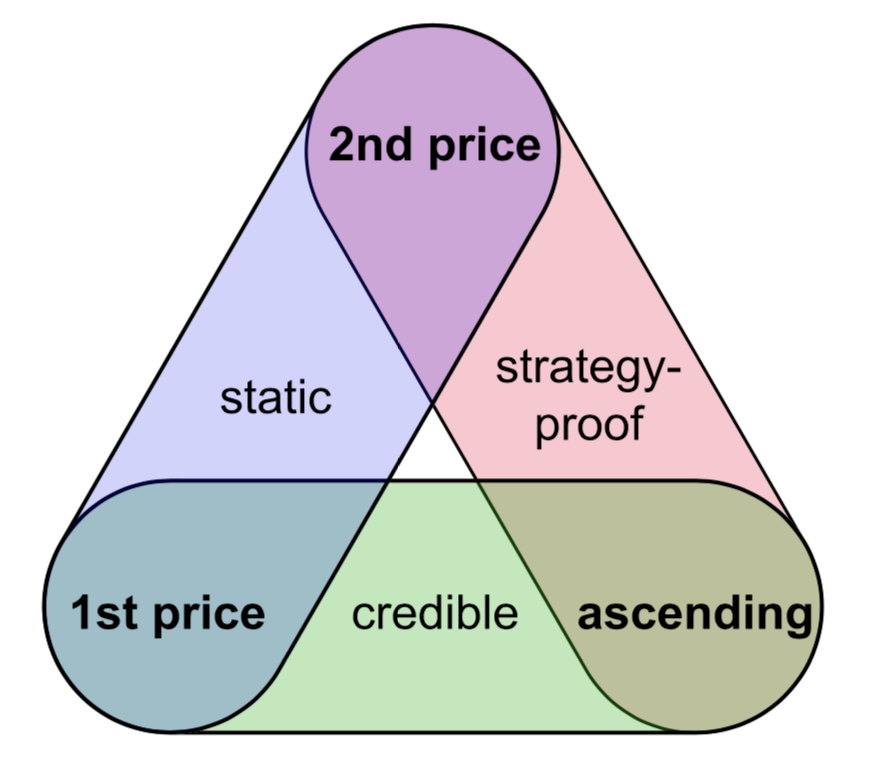
\includegraphics[height=5cm]{image/trilemma.png}
    \label{fig1}
\end{figure}

\subsection{Related Literature}
\paragraph{Almost the same concept, but restricted to direct (static) mechanisms}
\begin{itemize}
	\item Dequiedt and Martimort (2015, AER), Vertical contracting with informational opportunism.
	\item This paper: Extensive forms.
\end{itemize}

\paragraph{Commit to today's auction, not tomorrow's auction}
\begin{itemize}
	\item Milgrom 1987, mcAfee and Vincent 1997, Skreta 2015, Liu et al. 2017
	\item This paper: Not a repeated game.
\end{itemize}

\paragraph{Auctions as bargaining games}
\begin{itemize}
	\item McAdams and Schwarz 2007, Vartiainen 2013, Lobel and Paes Leme 2017
	\item This paper: No `red-handed' rule-breaking.
\end{itemize}


%%%
\newpage
\section{Model}
\begin{itemize}
	\item Agents: $i \in N$. A mechanism: an extensive game tree $G$. Outcomes: $X$.
	\item $\theta_N \sim \mD \in \Delta(\Theta_1, \dots, \Theta_N)$. Each type space is finite: $\Theta_i := \{\theta_i^1, \dots, \theta_i^{K_i}\}$.
	\item $S_i(I_i, \theta_i) \in A(I_i)$: agent $i$'s strategy. At each info. set, the set of possible action is finite.
	\item A protocol: $(G, S_N)$. Utiliry: $u_i: X \times \Theta_N \to \R$.
	\item agent $i$'s partition of the outcome space: $\mX_i$.
	\begin{itemize}
		\item e.g.) Each agent can observe only whether he makes a payment and receives the object.
	\end{itemize}
	\item $(G, S_N)$: BIC $\defi$ ... (as usual)
	\item Assume that $G$ is pruned. (This is w.l.o.g. when we consider credible and BIC mechanisms.)
\end{itemize}


\paragraph{Message games}
\begin{itemize}
	\item In each turn, CP either ends the game, or chooses some agent and send him a pair of a message and a set of acceptable replies $(m, R)$; then, the chosen agent sends CP a reply $r \in R$.
	\item Each agent's strategy: \{what they observed, current $R$\} $\to r \in R$.
	\item Agent $i$'s observation $o_i(S_0,S_N,\theta_N)$: communication sequence + cell of outcome partition.
\end{itemize}

\paragraph{The relationship between message games and mechanisms}
\begin{itemize}
	\item CP can run a protocol $(G, S_N)$ as a message game: $m := I_i$, $R := A(I_i)$.
	\item $S_0^G$: CP's strategy that runs the protocol $(G, S_N)$.
\end{itemize}
\begin{screen}
\begin{df}[Safe deviations] $G$: given.
	An observation $o_i(S_0, S_N, \theta_N)$ has an \textbf{innocent explanation} if
	\[
	\exists \theta'_{-i}; \ o_i(S_0, S_N, \theta_N) = o_i(S_0^G, S_N, (\theta_i, \theta'_{-i}))
	\]
	A CP's strategy $S_0$ is \textbf{safe} if $o_i(S_0, S_N, \theta_N)$ has an innocent explanation for all $i$ and $\theta_N$.
\end{df}
\end{screen}

\begin{itemize}
	\item $\mS_0^*(S_0^G, S_N)$: the set of safe deviations.
	\item As long as CP chooses a safe strategy, each agent cannot detect by himself that CP is cheating.
\end{itemize}

\paragraph{Credible mechanisms}
\begin{itemize}
	\item The protocol $(G, S_N)$ is credible if there is no profitable safe deviation for CP.
\end{itemize}
\begin{eg}
The trees below illustrates the mechanism that is not credible:
\begin{figure}[H]
  \centering
    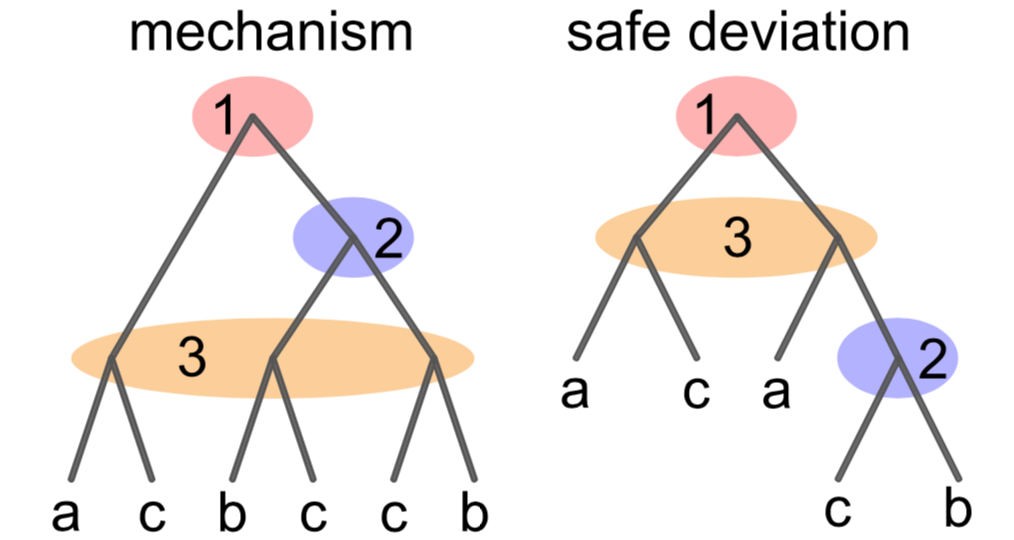
\includegraphics[height=4cm]{image/credible.png}
    \label{fig1}
\end{figure}
Assume that $\Omega_1 := \{\{a,b\}, \{c\}\}$, $\Omega_2 = \Omega_3 = \{\{a\}, \{b\}, \{c\}\}$, and $\theta_N := \{l_1, r_2, r_3\}$. 
If CP loves the outcome $a$, CP has a profitable safe deviation.
\end{eg}


\newpage
\section{Preliminary}
\begin{itemize}
	\item To use extensive forms, discretize Myerson 1981.
	\item In discrete settings, the analogue of continuous settings holds: the expected revenue is closely connected to virtual valuations.
	\item $u_i^{G, S_N}(k, k')$: the expected payoff of agent $i$ with his true type $\theta_i^k$ when he behaves as if his type is $\theta_i^{k'}$ under the protocol $(G, S_N)$.
\end{itemize}
\begin{df}[Virtual valuation, Regular distribution]
	\[
	\eta_i(\theta_i^k) := \left( \theta_i^k - \frac{1 - F_i(\theta_i^k)}{f_i(\theta_i^k)}\right)(\theta_i^{k+1} - \theta_i^k).
	\]
	\begin{itemize}
		\item $F_N := (F_i)_i$ is regular if $\eta_i$ is strictly increasing for all $i$. 
	\end{itemize}
\end{df}
\begin{df}[optimal mechanisms]
	The mechanism $(G, S_N)$ is optimal if it maximizes the expected revenue subject to the following conditions:
	\begin{itemize}
		\item IC: $(G, S_N)$ is BIC.
		\item Voluntary participation: $\forall i \exists S_i;$ $i$ does not win and has a zero transfer.
	\end{itemize}
\end{df}
\begin{prop}[Elkind(2007)] \label{optimal}
	$(G, S_N)$ is optimal iff
	\begin{enumerate}
		\item PCs bind for the lowest type: $\forall i; u_i^{G, S_N}(1, 1) = 0$.
		\item ICs bind locally downward: $\forall i \ \forall k \geq 2; \ u_i^{G, S_N}(k, k) = u_i^{G, S_N}(k, k-1)$.
		\item The allocation maximizes virtual value: $\forall \theta_N;$
		\begin{itemize}
			\item $\max_i \eta_i(\theta_i) > 0 \implies y^{G, S_N}(\theta_N) \in \argmax_i \eta_i(\theta_i)$.
			\item $\eta_i(\theta_i) < 0 \implies i \neq y^{G, S_N}(\theta_N)$.
		\end{itemize}
	\end{enumerate}
	
	If $(G, S_N)$ is optimal, its expected revenue coincides with the expected virtual valuation of the winner: \ocomment{[要確認]}
	\[
	\pi(G, S_N) = \E_{\theta_n} \left[ \sum_{i \in N} y^{G, S_N}(\theta_N) \eta_i(\theta_i) \right]
	\]
\end{prop}

\begin{prop}[the expected revenue $\simeq$ the expected virtual value] \label{bound}
	If $(G, S_N)$ is BIC, then
	\[
	0 \leq 
	\E_{\theta_n} \left[ \sum_{i \in N} y^{G, S_N}(\theta_N) \eta_i(\theta_i) \right]
	- \pi(G, S_N)
	- \sum_{i \in N} u_i^{G, S_N}(1, 1)
	\leq \max_i \max_{2 \leq k \leq K_i} \{\theta_i^k - \theta_i^{k-1}\}
	\]
\end{prop}


%%%
%\newpage
\section{Results}
\begin{ass}
	$F_N$: regular, symmetric. Auctions are winner-paying. $\theta_1 \leq 0$. $\theta^1 < \dots < \theta^K$. 
\end{ass}

\subsection{Quasi-FPAs and credible static auctions.}
\begin{df}[quasi-FPA]
	A quasi-FPA is a static mechanism that can have at most one special agent. If there is no special agent, it is a normal FPA. If there is a special agent $i^*$ with a posted price $p^*$, he can surely win if he bids $p^*$. (NB: Even if $p^*$ is not the highest bid among all bidders, CP should allocate the object to $i^*$.)
\end{df}

\begin{screen}
\begin{thm}[The characterization of credible and static auctions.] \label{thm_fpa}
	Suppose the auction $(G, S_N)$ is BIC and winner-paying. Then,
	\[
	\text{$(G, S_N)$ is credible and static $\equi$ $(G, S_N)$ is a quasi FPA.}
	\]
	%Note that this implies $\{\text{credible and static auctions}\} = \{\text{quasi FPAs}\} \supset \{\text{FPAs}\}$, assuming the mechanisms we are considering are BIC and winner-paying.
\end{thm}
\end{screen}


\begin{proof}
	$\Leftarrow)$: Easy.
	\paragraph{$\Rightarrow)$}
	First, observe that if the mechanism is credible and agent $i$ have chances to win when he chooses an action $a$, the possible payment is uniquely determined; otherwise CP can improve his payoff safely. Hence, each action corresponds to a unique payment $b_i(a)$, and it can be regarded as agent $i$'s bid.
	\paragraph{Case (i): There is a special agent $i^*$ with a posted price $p^*$, and $i^*$ bids $p^*$.}
	If there is a special agent $i^*$, who can surely obtain the object if he bids $p^*$. Suppose $i^*$ bids $p^*$. CP should allocate the object to $i^*$; there is no profitable safe deviation for CP. This is a quasi-FPA.
	(NB: Since the protocol is BIC, $p^* := \max_{a \in A(I_i)} b_i(a)$.)
		
	\paragraph{Case (ii): There is no special agent, or $i^*$ does not bid $p^*$.}
	In this case, it is best for CP to allocate the object to the highest bidder. This is also a (quasi-)FPA.
\end{proof}

\begin{screen}
\begin{prop}[There is an almost-optimal FPA. $p^*$ cannot be very low.] \label{prop_q-fpa}
	Let $\epsilon := \max_{2 \leq k} \{\theta^{k} - \theta^{k-1}\}$.
	\begin{itemize}
		\item There is an $\epsilon$-optimal FPA with reserve $\rho^* := \min_k \{\theta^k \mid \eta_i(\theta^k) > 0\}$.
		\item If a quasi-FPA is BIC and maximizes virtual value, then $p^*$ (if it exists) is at least $\max_i b_i(S_i(I_i, \theta^{K-2}))$.
	\end{itemize}
\end{prop}	
\end{screen}

\begin{proof}
	Note that we need to construct a set of feasible actions in a quasi-FPA with reserve $\rho^*$ so that $(G, S_N)$ is $\epsilon$-optimal.
	
	First, consider the SPA with reserve $\rho^*$. It is best for each agent to bid truthfully. Let $\bar{b}_i(\theta_i)$ be the payment for type $\theta_i$ agent conditional on winning. (If agent $i$ never wins with type $\theta_i$, $\bar{b}_i(\theta_i) := -1$.)
	
	Next, we construct the desirable FPA $G$ with reserve $\rho^*$. Let $\bar{b}_i(\theta_i) \in A(I_i)$. Suppose that every agent $i$ bid $\bar{b}_i(\theta_i)$. In this case, the strategy profile $S_N := (\bar{b}_i(\theta_i))_{i \in N, \theta_i \in \Theta_i}$ is BIC under $G$; otherwise, in a SPA with a sufficiently fine action space, there is a profitable deviation that allows an agent to obtain strictly better payoff compared to the payoff he can obtain under truthful bidding. Note that, in $(G, S_N)$, PCs for the lowest types bind.
	
	Observe that $(G, S_N)$ maximizes the expected virtual value, though $G$ may not satisfy the locally downward ICs condition. Then, by Prop.\ref{bound}, 
	\[
	0 \leq 
	\underbrace{\E_{\theta_n} \left[ \sum_{i \in N} y^{G, S_N}(\theta_N) \eta_i(\theta_i) \right]}_{\text{the exp. rev. under the opt. auctions}}
	- \underbrace{\pi(G, S_N)}_{\text{the exp. rev. under $(G, S_N)$}}
	\leq \max_{2 \leq k \leq K_i} \{\theta_i^{k} - \theta_i^{k-1}\}
	\]
	
	The second part follows from the symmetry of $F_N$ and BIC.
\end{proof}



%%%
\subsection{Ascending auctions and credible strategy-proof auctions.}
\begin{df}[Ascending auctions]
	(omitted.)
\end{df}
\begin{screen}
\begin{thm}[credible + SP = AA, assuming the auction is optimal]
	Assume the protocol $(G, S_N)$ is optimal. Then,
	\[
	\text{$(G, S_N)$ is credible and strategy-proof $\equi$ $(G, S_N)$ is an AA.}
	\]
\end{thm}
\end{screen}


\begin{proof}[Sketch of the proof.]
	\textbf{ $\Leftarrow)$}
	Assume $(G, S_N)$ is an AA. SP is ok. Suppose toward contradiction that $(G, S_N)$ is not credible. Then, there is a profitable safe deviation for CP $S_0'$. Observe that $S_N$ is a best reply even if CP announces that he will commit to $S_0'$, that is, for all agent $i$, the mechanism proceeds as if the other agents' types are different from the reported ones. The corresponding protocol $(G', S_N')$ has strictly higher expected revenue than $(G, S_N)$; this contradicts the optimality of $(G, S_N)$.
	
	\paragraph{$\Rightarrow)$}
	One major feature of AA: at each history, the action of all types' that might win in the future pools. If their action does not pool, CP has a profitable safe deviation. (To show this statement, they develop a smart algorithm.)
\end{proof}

\subsection{The Auction Trilemma}
\begin{screen}
\begin{cor}[The Auction Trilemma] \label{trilemma}
Assume $F_N$ is regular and symmetric, and $(G, S_N)$ is BIC and winner-paying.
	\begin{enumerate}
		\item Suppose there exists $i$ and $\theta_i, \theta_i'$ such that $t_i^{G, S_N}(\theta_i) > t_i^{G, S_N}(\theta_i') \geq 0$. If $(G, S_N)$ is optimal, it cannot be static, credible and strategy-proof at the same time.
		\item Let $\epsilon := \max_{k \geq 2} \{\theta^k - \theta^{k-1}\}$. There exist $\epsilon$-optimal auctions with some reserve $\rho^*$ that satisfy one of the following properties:
		\begin{itemize}
			\item static and strategy-proof (SPA)
			\item static and credible (FPA)
			\item strategy-proof and credible (AA)
		\end{itemize}
	\end{enumerate}
\end{cor}
\end{screen}

\begin{proof}
	We can show the second part by the same argument as in Prop.\ref{prop_q-fpa}: Observe that, with reserve $\rho^* := \max_i\{\theta^k \mid \eta_i(\theta^k) > 0\}$, these auctions maximize the virtual value of winner, and PC for the lowest types bind.
	
	\paragraph{The first part:}
	By Thm.\ref{thm_fpa}, if the auction is static and credible, it is a quasi-FPA. By the assumption, $i$ has no less than two possible bids; each bid should win with positive probability because we consider pruned mechanisms. Therefore, for some type profile, $i$ can win by the lower bid; strategy-proofness cannot hold.
\end{proof}

\begin{cor}[Strategy-proofness holds only for one side.]
	Assume $F_N$: regular and symmetric, and $(G, S_N)$ is orderly and optimal. Suppose the optimal reserve $\rho^* < \theta^{K-2}$. In the messaging game restricted to $\mS_0^*(S_0^G, S_N)$, either of the followings holds:
	\begin{enumerate}
		\item $\exists S_N';$ $S_0^G$ is not a BR to $S_N'$.
		\item $\exists i \in N \ \exists S'_{N \setminus \{i\}};$ $S_i$ is not BR to $(S_0^G, S'_{N \setminus \{i\}})$.
	\end{enumerate}
\end{cor}
\begin{proof}
	\textbf{Case (i) $(G, S_N)$ is not credible:} For $S_N$, $S_0^G$ is not BR. (The first one holds.)
	
	\noindent
	\textbf{Case (ii) $(G, S_N)$ is not strategy-proof:} The second one holds.
	
	\noindent
	\textbf{Case (iii) $(G, S_N)$ is credible and strategy-proof:}
	Since it is optimal, it is an AA. Fix some $i$ and consider the strategy profile such that $i$ stays until the price hits $\theta^K$ and other agents quits before the reserve is met. CP apparently has a profitable safe deviation.
	
\end{proof}







\end{document}